\documentclass{bmcart}

%%%%%%%%%%%%%%%%%%%%%%%%%%%%%%%%%%%%%%%%%%%%%%
%%                                          %%
%% CARGA DE PAQUETES DE LATEX               %%
%%                                          %%
%%%%%%%%%%%%%%%%%%%%%%%%%%%%%%%%%%%%%%%%%%%%%%

%%% Load packages
\usepackage{amsthm,amsmath}
\usepackage{graphicx}
%\RequirePackage[numbers]{natbib}
%\RequirePackage{hyperref}
\usepackage[utf8]{inputenc} %unicode support
%\usepackage[applemac]{inputenc} %applemac support if unicode package fails
%\usepackage[latin1]{inputenc} %UNIX support if unicode package fails


%%%%%%%%%%%%%%%%%%%%%%%%%%%%%%%%%%%%%%%%%%%%%%
%%                                          %%
%% COMIENZO DEL DOCUMENTO                   %%
%%                                          %%
%%%%%%%%%%%%%%%%%%%%%%%%%%%%%%%%%%%%%%%%%%%%%%

\begin{document}

	\begin{frontmatter}
	
		\begin{fmbox}
			\dochead{Biología de Sistemas}
			
			%%%%%%%%%%%%%%%%%%%%%%%%%%%%%%%%%%%%%%%%%%%%%%
			%% INTRODUCIR TITULO PROYECTO               %%
			%%%%%%%%%%%%%%%%%%%%%%%%%%%%%%%%%%%%%%%%%%%%%%
			
			\title{Trombosis Arterial}
			
			%%%%%%%%%%%%%%%%%%%%%%%%%%%%%%%%%%%%%%%%%%%%%%
			%% AUTORES. METER UNA ENTRADA AUTHOR        %%
			%% POR PERSONA                              %%
			%%%%%%%%%%%%%%%%%%%%%%%%%%%%%%%%%%%%%%%%%%%%%%
			
			\author[
			  addressref={aff1},                   % ESTA LINEA SE COPIA IGUAL PARA CADA AUTOR
			  corref={aff1},                       % ESTA LINEA SOLO DEBE TENERLA EL COORDINADOR DEL GRUPO
			  email={pablomolinasanchez01@uma.es}   % VUESTRO CORREO ACTIVO
			]{\inits{P.M.S}\fnm{Pablo} \snm{Molina Sánchez}} % inits: INICIALES DE AUTOR, fnm: NOMBRE DE AUTOR, snm: APELLIDOS DE AUTOR
			\author[
			  addressref={aff1},
			  email={hugoavalos@uma.es}
			]{\inits{H.A.R}\fnm{Hugo} \snm{Ávalos de Rorthais}}
			
			%%%%%%%%%%%%%%%%%%%%%%%%%%%%%%%%%%%%%%%%%%%%%%
			%% AFILIACION. NO TOCAR                     %%
			%%%%%%%%%%%%%%%%%%%%%%%%%%%%%%%%%%%%%%%%%%%%%%
			
			\address[id=aff1]{%                           % unique id
			  \orgdiv{ETSI Informática},             % department, if any
			  \orgname{Universidad de Málaga},          % university, etc
			  \city{Málaga},                              % city
			  \cny{España}                                    % country
			}
		
		\end{fmbox}% comment this for two column layout
		
		\begin{abstractbox}
		
			\begin{abstract} % abstract
			Artículo en el que explicamos la trombosis arterial, desde la breve descripción de la enfermedad hasta la investigación de los mecanismos moleculares subyacentes a la enfermedad. Para ello hemos utilizado un HPO (0004420, Arterial thrombosis) explicando a nivel de gen cuáles intervienen en el desarrollo de la enfermedad, de mayor a menor importancia. También vemos algunas enfermedades asociadas a la trombosis que se relacionan por tener numerosos genes en común.
			%%%%%%%%%%%%%%%%%%%%%%%%%%%%%%%%%%%%%%%%%%%%%%%
			%% RESUMEN BREVE DE NO MAS DE 100 PALABRAS   %%
			%%%%%%%%%%%%%%%%%%%%%%%%%%%%%%%%%%%%%%%%%%%%%%%	
			
			\end{abstract}
			
			%%%%%%%%%%%%%%%%%%%%%%%%%%%%%%%%%%%%%%%%%%%%%%
			%% PALABRAS CLAVE DEL PROYECTO              %%
			%%%%%%%%%%%%%%%%%%%%%%%%%%%%%%%%%%%%%%%%%%%%%%
			
			\begin{keyword}
			\kwd{gen}
			\kwd{enfermedad}
			\kwd{mecanismo molecular}
			\end{keyword}
		
		
		\end{abstractbox}
	
	\end{frontmatter}
	
	%%%%%%%%%%%%%%%%%%%%%%%%%%%%%%%%%%%%%%%%%%%%%%%%%%%%%%%%%%%%%%%%%%%%%%%%%%%%%%%%%%%%%%%%
	%% EJEMPLO DE LATEX %%                                                                %%
	%% BORRAR ANTES DE ENTREGAR!!!!!!!!!!!!!!!!!!!!!!!!!!!!!!!!!!!!!!!!!!!!!              %%
	%%%%%%%%%%%%%%%%%%%%%%%%%%%%%%%%%%%%%%%%%%%%%%%%%%%%%%%%%%%%%%%%%%%%%%%%%%%%%%%%%%%%%%%%

	
	\section*{Introducción}
	
La formación de un trombo en el interior de una arteria se denomina trombosis arterial. Esta formación de coágulos suele desencadenarse con la ruptura de una placa ateroesclerótica \cite{Trombosis_Bayer}. Una placa ateroesclerótica (figura \ref{fig:Figura 1}, área amarilla) es la manifestación principal de la aterosclerosis, que no es más que la acumulación de grasas, colesterol y otras sustancias dentro de las arterias y en sus paredes \cite{Aterosclerosis_inflamacion}. La ruptura de estas placas es un acontecimiento que provoca un entorno favorable a la formación de trombos, al que se incorporan rápidamente las plaquetas (figura \ref{fig:example1}, adelgazamiento del vaso).

\begin{figure}[h]
    \centering
	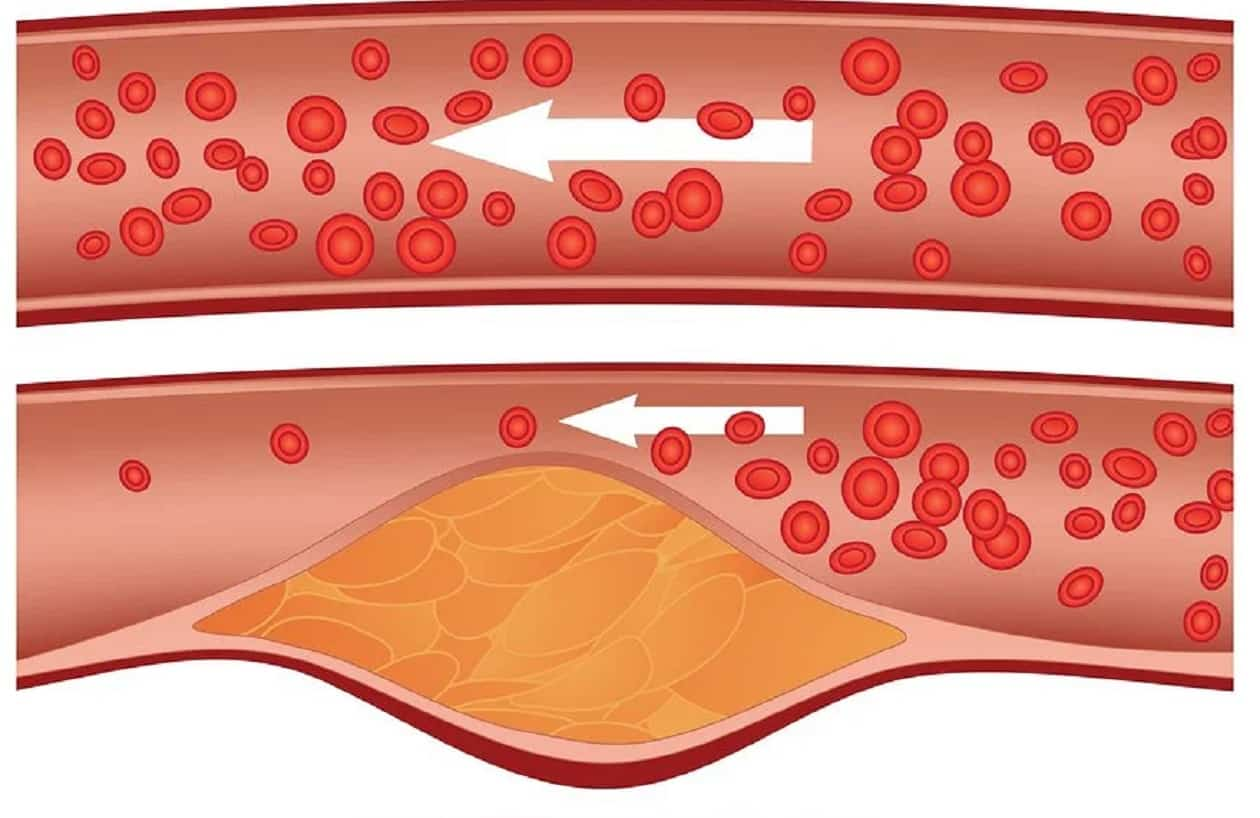
\includegraphics[width=0.70\textwidth]{figures/aterosclerosis.jpg}
	\caption{Formación de un trombo por aterosclerosis. La imagen nos muestra la formación de trombos arteriales provocados por aterosclerosis. En amarillo podemos ver las placas ateroscleróticas impidiendo el paso del flujo arterial en rojo (tomado de \cite{imagen_trombo})}
	\label{fig:Figura 1}
  \end{figure}
  
La incorporación de plaquetas al trombo provoca que la cantidad de fibrina aumente puesto que actúa como una especie de pegamento o hilo entre las plaquetas. Así, el coágulo aumenta lentamente a medida que el trombo se extiende por la luz arterial. Por ello, un trombo arterial contiene generalmente muchas plaquetas y aumenta rápidamente de tamaño \cite{Aterosclerosis_inflamacion} \cite{Trombosis_Bayer}
Los trombos asociados a la arritmia se forman en entornos de bajo flujo y baja presión, por lo que los coágulos resultantes crecen lentamente y son ricos en fibrina. También se clasifican como trombos arteriales, aunque se asemejan más a los trombos de tipo venoso, cumpliendo así la tríada de Virchow \cite{Triada_Virchow}) para la trombogénesis: Lesión endotelial, Lentitud del flujo y Estado de hipercoagulabilidad
\\

Este tipo de coágulo sanguíneo puede causar ataques cardiacos bastante graves, si el taponamiento es en las arterias coronarias, o accidentes cerebrovasculares (en ocasiones irreversibles), si el taponamiento es en arterias cerebrales. La trombosis arterial es muy dañina para el organismo y, en general, mucho más grave y urgente que la trombosis venosa debido a la falta de oxígeno que provoca el taponamiento de las arterias en aquellos lugares donde están ubicadas \cite{Trombosis_Bayer}. 
	
\subsection{Genes Asociados}
		La trombosis arterial se ve afectada por diversos genes. Este mapa nos muestra las interacciones entre los 25 genes que intervienen ).
		
    \begin{figure}[h]
        \centering
    	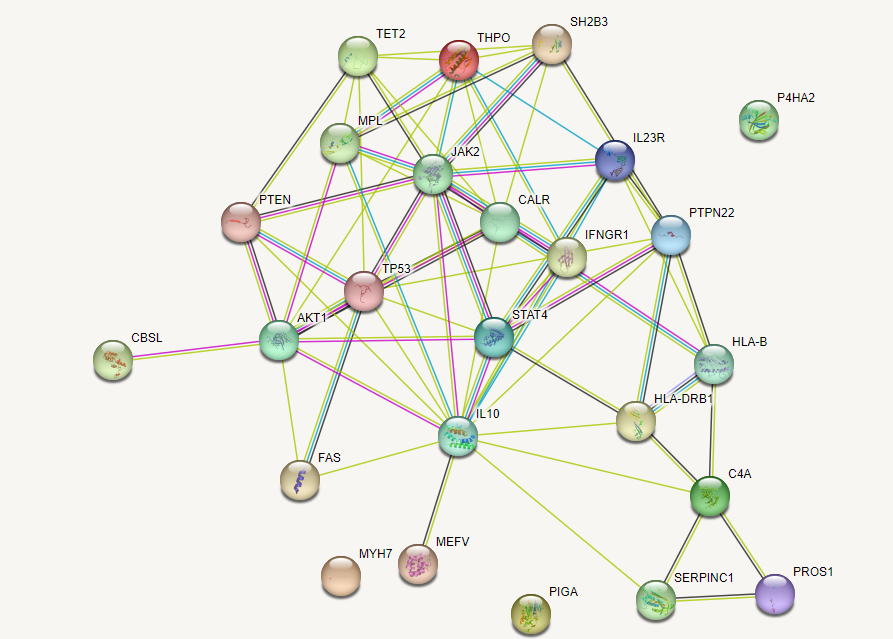
\includegraphics[width=0.70\textwidth]{figures/genes_asociados.png}
    	\caption{Genes asociados en la trombosis. La imagen nos representa los genes asociados a la trombosis arterial en círculos con sus respectivos nombres. Además también nos representa las iteracciónes entre ellos en líneas de colores (tomada de \cite{grafo}.}
    	\label{fig: Figura 2}
      \end{figure}
\subsubsection{JAK2, STAT4 e IL10}

          El gen JAK2 es relevante, ya que como podemos ver en la Figura \ref{fig: Figura 2}  participa en multitud de interacciones entre genes. Para explicar el funcionamiento de este gen es necesario explicar las quinasas Janus, tipología de la JAK2.\\
		
		Las quinasas Janus están en el origen de diversas respuestas inmunológicas e inflamatorias y engloban 4 enzimas intracelulares de tipo tirosina-quinasa (JAK1, JAK2, JAK3 y TYK2 [tyrosine kinase-2]). En este caso, la que interviene en la trombosis es la JAK2 \cite{JAK2}. Estas enzimas están asociadas con la región membranosa intracelular de distintos receptores que convierten las señales extracelulares, mediadas por diversas citocinas u hormonas, en procesos intracelulares \cite{JAK2}. La unión de una citosina al receptor causa su dimerización e induce la activación de las JAK asociadas. Cuando esto ocurre, las JAK fosforilan residuos específicos del dominio citoplasmático del receptor, donde se anclan los transductores de señales (STAT) \cite{JAK2}. Entonces se produce la fosforilación de los STAT que una vez activados se dimerizan y traslocan al núcleo, donde participan en la expresión de múltiples proteínas \cite{JAK2} \cite{STAT4}.\\
		
		Esta proteína es esencial para mediar las respuestas a la IL10 en los linfocitos, que es una citocina reguladora del sistema inmunitario que actúa sobre muchas células con propiedades antiinflamatorias, capaz de inhibir la síntesis de citocinas proinflamatorias por los linfocitos T y los macrófagos \cite{IL10}). STAT4 también regula la diferenciación de las células T helper, además de ser de suma importancia en la regulación del equilibrio entre ambas \cite{STAT4} . La deficiencia de STAT4 da lugar a una reducción de la aterosclerosis a través de la modulación de la función de las células B y del contenido de leucocitos en la aorta. Esta respuesta inmunológica hacia la anomalía de la arterosclerosis, provoca el aumento de leucocitos favoreciendo el taponamiento de glóbulos rojos \cite{STAT4}). Es por ello, que las trombosis arteriales también son denominadas blancas.\\

	
	

\subsection{Enfermedades Asociadas}
La trombosis arterial en ocasiones provoca problemas de salud más graves. Uno de ellos es la \textbf{Trombosis Familiar}, la cual es un tipo de trombosis que afecta a la línea de progenitores de plaquetas/megacariocitos y puede producir tendencia a trombosis y hemorragia, pero no causa proliferación maligna \cite{Trombocitosis_Familiar}.\\
También puede provocar un \textbf{Trombocitemia Esencial} que  es uno de los trastornos mieloproliferativos Ph-negativos más frecuentes. Esta se caracteriza por una elevación mantenida de las plaquetas, debida a la proliferación excesiva de los megacariocitos de la médula ósea \cite{Trombocitema_Esencial}.\\
Por último, otra enfermedad común es la \textbf{Policitemia Vera}, que es un síndrome mieloproliferativo de carácter adquirido. Está caracterizada por un aumento absoluto de la masa eritrocitaria debido a su proliferación incontrolada que generalmente se asocia a una proliferación, también incontrolada de leucocitos y plaquetas \cite{Policitema_Vera}.


	\section*{Materiales y métodos}
	\section{Materiales y métodos}

\subsection{Materiales}

En esta sección vamos a explicar las librerías de R más significativas y otros recursos que hemos usado durante el proyecto.

\subsubsection{Human Phenotype Ontology}

HPO (Human Phenotype Ontology)\cite{HPO} es un vocabulario estandarizado de anomalías fenotípicas en enfermedades humanas que utiliza un fenotipado preciso y detallado para poder ser usado a nivel computacional en distintos campos de la medicina.


\subsubsection{StringDB}

STRING (Search Tool for the Retrieval of Interacting Genes/Proteins) \cite{STRING} es una base de datos biológica sobre interacciones entre proteínas, tanto interacciones conocidas como previstas. Estas interacciones incluyen tanto asociaciones directas como indirectas.

\subsubsection{ClusterProfiler}

Paquete de R que proporciona diferentes funciones para el análisis funcional de genes.

\subsubsection{igraph}

Es una librería diseñada para la investigación en la ciencia de redes. Esta que nos permite crear, manipular y analizar redes y gráficos. Se puede usar con lenguajes de alto nivel como R y Python.

\subsubsection{Linkcomm}

 Las comunidades nos dan información sobre la estructura y las conexiones que forman los diferentes nodos de una red, pudiendo así identificar aquellos que forman conexiones con múltiples comunidades. Linkcomm \cite{linkcomm} nos proporciona herramientas para generar y manipular estas comunidades sin importar su tamaño y tipo.



\section{Métodos}

En este apartado se explicará los diferentes métodos que se han seguido a lo largo del proceso de análisis de la formación de un trombo arterial investigando las interacciones entre los genes que intervienen en la enfermedad.

\subsection{Obtención de proteínas y genes asociados}

El primer paso fue obtener los genes participantes en la trombosis arterial. Para ello primero tuvimos que apoyarnos en el \textit{HPO} de la enfermedad \cite{HPO} para obtener el listado de 25 genes. Posteriormente, nos apoyamos en la web de \textit{STRING} \cite{STRING} , en la que, tras pasar como parámetro el conjunto de genes anterior, obtuvimos una representación gráfica de las interacciones entre los 25 genes. El resultado obtenido fue el mostrado en la figura \ref{fig: Figura 2}. También desde STRING obtuvimos las interacciones entre genes y el grado de cada uno de ellos, los cuales utilizaremos posteriormente para el desarrollo del código. Se comentará más adelante en la sección \textit{Generación de análisis de red PPI}. \\



\subsection{Generación y análisis de red PPI}
Una vez obtenido los genes participantes en la trombosis arterial, comenzamos con nuestro análisis de red PPI. Para ello, primeramente hemos creado el grafo con los genes asociados y realizado un \textit{análisis del grado} con las funciones del paquete \textit{igraph} \cite{igraph}. 

Tras el análisis del grado, hemos llevado a cabo una \textbf{propagación de genes} a través de \textit{STRING} \cite{STRING}, para mejorar la conectividad de la red, además de evitar que posibles genes se encuentren desconectados de nuestro sistema a estudiar, haciendo que los análisis que realicemos sean más esclarecedores, ya que tenemos una mejor visión del contexto de la enfermedad. 

Tras esto, hemos utilizado el paquete \textit{linkcomm} \cite{linkcomm} para llevar a cabo un \textbf{análisis de las comunidades del sistema}, pudiendo determinar los genes que conectan comunidades, así como el tamaño de ellas entre otros distintos análisis que explicaremos en profundidad en la sección \textit{Resultados} .

Por último, hemos llevado a cabo un \textbf{análisis funcional} mediante el enriquecimiento con GO del paquete \textit{clusterProfiler} \cite{clusterProfiler} de los procesos biológicos en los que intervienen los genes integrantes de cada una de las distintas comunidades anteriormente obtenidas, apoyándonos en el conjunto genómico del \textit{Homo Sapiens Sapiens} del paquete \textit{DOSE} \cite{DOSE}.  Así, hemos obtenido las distintas funciones biológicas que se llevan a cabo en el proceso de la trombosis arterial, además de poder mostrar que genes son partícipes de cada una de las fases de formación del trombo.

	\section*{Resultados}
	 \newpage
 \section{Resultados}
 
 \subsection{HPO}
 Esta enfermedad, Trombosis Arterial, está definida como HPO:0004420, manteniendo relación con otras 26 enfermedades y con 25 genes asociados.
 
 \subsection{STRING}
 Con la base de datos biológica \textit{STRING} \cite{STRING}, hemos obtenido los genes asociados y sus interacciones.
 
 \begin{minipage}{\linewidth}
 	\makebox[\linewidth]{
		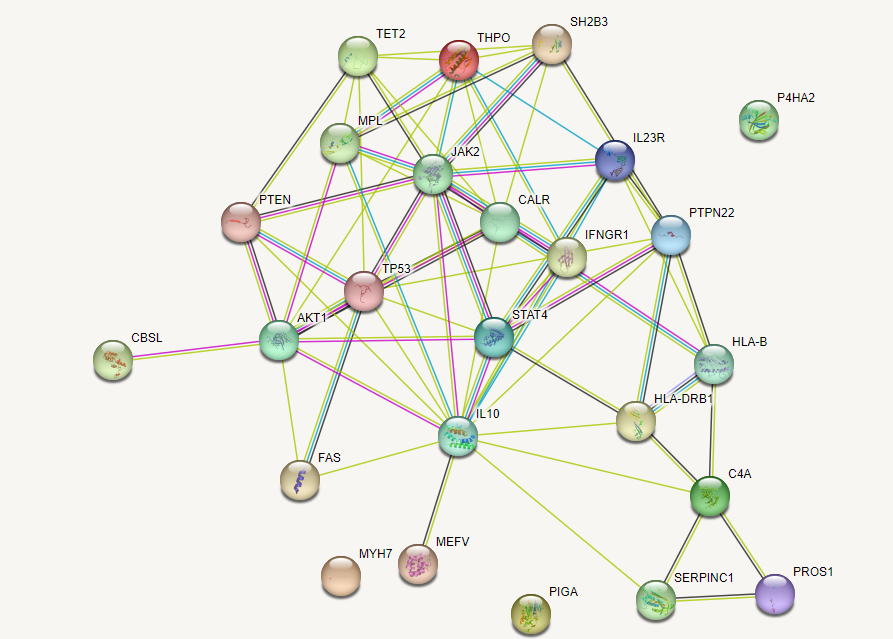
\includegraphics[width=0.70\textwidth]{figures/genes_asociados.png}

 	}
 	\captionof{figure}{Genes asociados a la trombosis.}
 	\label{fig: Figura 3}
 \end{minipage}



\subsection{Comunidades}
Con la propagación de genes en \textit{STRING} hemos obtenido el siguiente grafo de 70 genes (45 semillas).

 \begin{minipage}{\linewidth}
	\makebox[\linewidth]{
	 	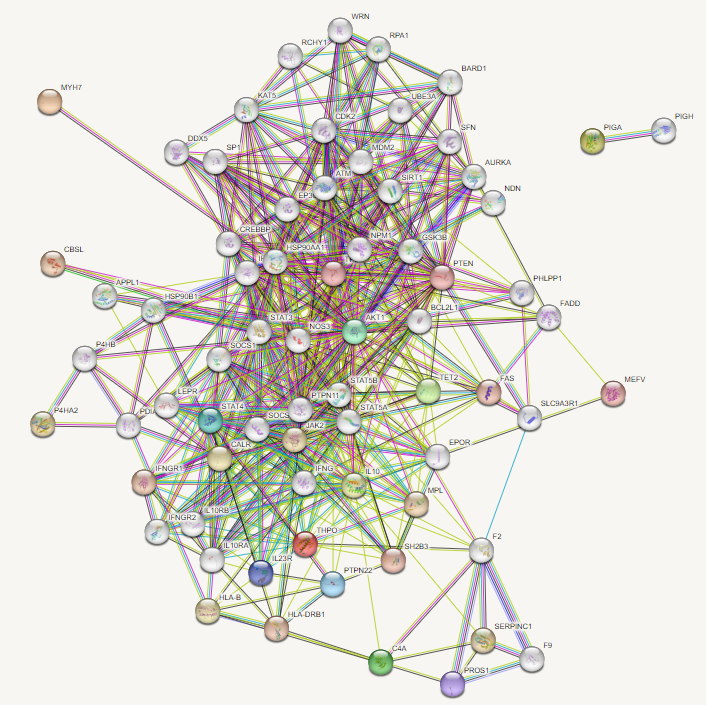
\includegraphics[width=0.70\textwidth]{figures/network_propagation.png}
		
	}
	\captionof{figure}{Conjunto de genes tras la propagación, siendo los de color gris genes semilla y los de color los iniciales representados en la figura \ref{fig: Figura 3}.}
	\label{fig: Figura 4}
\end{minipage}

\begin{spacing}{1}
Se han obtenido un total de 18 comunidades genéticas, con el paquete \textit{linkcomm}, representadas en la figura 5. Vemos que la comunidad morada es la comunidad más amplia. 
\end{spacing}

\begin{minipage}{\linewidth}
	\makebox[\linewidth]{
		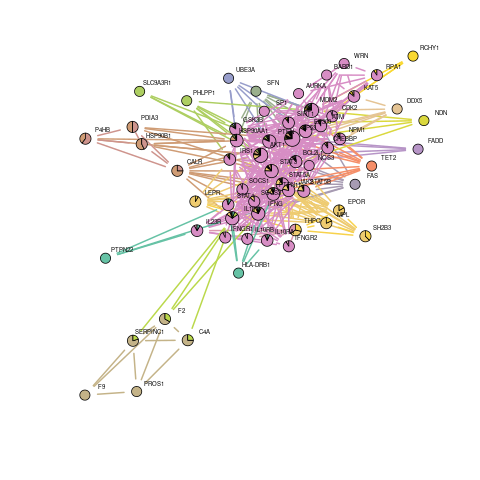
\includegraphics[width=1\textwidth]{figures/01_NetworkComunidades.png}
		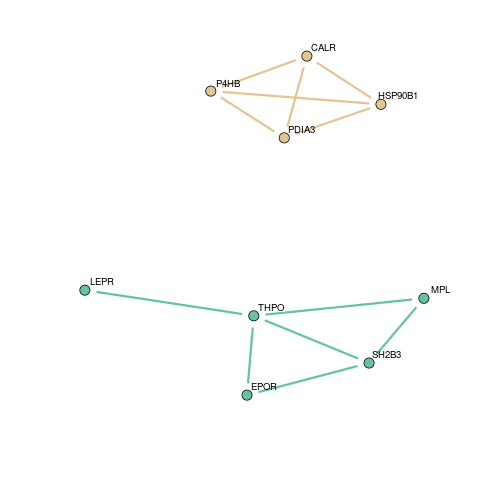
\includegraphics[width=0.70\textwidth]{figures/05_Comunidades_Independientes.png}
		
	}
	\captionof{figure}{Comunidades genéticas generadas con el paquete \textit{linkcomm} al conjunto de genes representados en la figura  \ref{fig: Figura 4}.}
	\label{fig: Figura 5}
\end{minipage}

\begin{spacing}{1}
También podemos ver las comunidades independientes de nuestro reactoma. En nuestro caso, las comunidades independientes son dos y estarían conformadas por un lado por \textit{P4HB, PDIA3, CALR, HSP90B1} y por otro lado por \textit{LEPR, THPO, MPL, SH2B3, EPOR}
\end{spacing}


\begin{spacing}{1}
	A continuación, en la figura \ref{fig: Figura 7} podemos ver una matriz con los genes que unen y, por tanto, pertenecen a más comunidades. En nuestro caso, podemos observar que los genes TP53 y AKT1 son los genes que unen y pertenecen a más comunidades con 10 y 8 conexiones respectivamente, marcado a la derecha. En la parte posterior del gráfico nos indica las comunidades a las que pertenecen estos genes, colocándose en la parte inferior la sumatoria de las comunidades a las que pertenecen estos diez genes. Vemos, que todos son parte de la comunidad 16.
\end{spacing}



\begin{minipage}{\linewidth}
	\makebox[\linewidth]{
		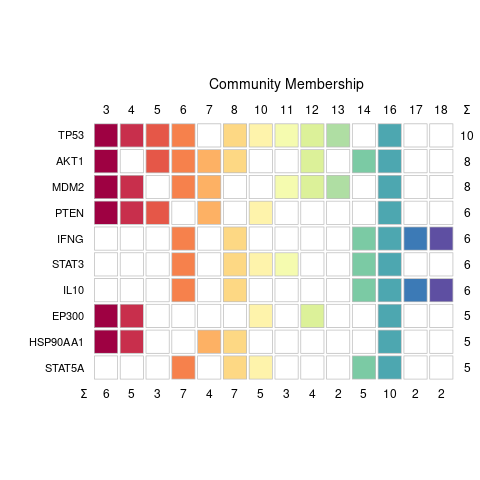
\includegraphics[width=0.70\textwidth]{figures/03_GenesMasCOnectadosOtrasComunidades.png}
		
	}
	\captionof{figure}{Genes que unen comunidades}
	\label{fig: Figura 7}
\end{minipage}



\subsection{Análisis funcional de las comunidades}
Se ha realizado el análisis funcional a todas las comunidades, los ficheros .csv resultantes se pueden visualizar en el GitHub en la carpeta 'results'.


	\section*{Siscusión}
	\section{Discusión}
\hfill


\hfill

Respecto a los genes que unen comunidades, graficados en la figura \ref*{fig: Figura 7} vemos al \textbf{TP53} y \textbf{AKT1} como los genes que pertenecen a más comunidades. El gen TP53 es un regulador la división celular impidiendo que las células crezcan y se dividan (proliferen) demasiado rápido o de forma incontrolada \cite{TP53}. Por tanto, sabiendo su función, podemos afirmar que tiene un papel regulador en los procesos biológicos de todas y cada una de las comunidades a las que pertenece. Este sería el motivo por el que une tantas comunidades, además de ser el motivo por el que adquiere gran importancia en el reactoma.\\\\  A su vez, el gen AKT1 proporciona instrucciones para fabricar una proteína denominada quinasa AKT1 \cite{AKT1}. Esta proteína se encuentra en varios tipos de células de todo el organismo, donde desempeña un papel fundamental en muchas vías de señalización \cite{AKT1}. Por tanto, este sería el motivo por el que une tantas comunidades y, al igual que TP53, adquiere especial relevancia en el estudio.\\\\
Ambos pertenecen a la \textit{comunidad 16}, comunidad de mayor tamaño del reactoma. Esta comunidad interviene en cualquier proceso que provoque un cambio en el estado del organismo. En nuestro caso, nos referimos al pathway \textbf{JAK-STAT}, nombrado en \textit{Genes Asociados} y mediante el cual obtenemos las células T-helper \cite{pathway}, que provoca que los linfocitos B liberen anticuerpos hacia la placa aterosclerótica, interpretada como cuerpo extraño.\\\\
En consonancia nuevamente con la introducción y los resultados funcionales de las comunidades, hemos podido observar que adquiere gran importancia en la enfermedad la \textit{comunidad 1}. A raíz de el artículo recomendado \cite{F2_F9} por la base de datos STRING \cite{STRING}  y nuestro resultado del análisis funcional de la \textit{comunidad 1}, hemos podido observar la importancia en la enfermedad de un gen en concreto, el gen \textbf{F2}, el cual es activado por el gen \textbf{F9}. Este gen F2 es el encargado de sintetizar \textit{protrombina}, inofensiva hasta que ocurre un daño, donde se convierte en la \textit{trombina}, su forma activa. Esta trombina convierte el fibrinógeno en fibrina, que juega un papel muy importante en la formación y proceso trombótico como hemos explicado en la sección \textit{Introducción}. También, perteneciente a esta comunidad hemos visto el gen \textbf{SERPINC1}, que sintetiza la \textit{antitrombina}, un inhibidor de la trombina \cite{SERPINC1}. Una mutación en este gen provocaría un aumento del riesgo de eventos trombóticos. Si por alguna otra causa también muta el gen F2 y aumenta su actividad, tendríamos un entorno muy favorable a la formación de trombos.\\\\
También perteneciente a esta comunidad, tenemos el \textbf{PROS1}, que sirve como cofactor de la proteína C activada de tipo 4, cuyo pathway de formación es iniciado por el gen \textbf{C4A} \cite{PROS1}. Estos dos genes, intervienen en la inactivación proteolítica de factores de coagulación que el cuerpo para su eliminación a través de células inmunitarias. Por tanto, tratan de eliminar el resultado de la sintetización de la protrombina de la F2.\\\\ Esta comunidad interviene en la coagulación a través de mutaciones en el gen F2 y SERPINC1, que provocan la saturación e inoperancia de los genes PROS1 y C4A en su intento por eliminar ese desorden homeostático de fibrina.\\\\
Por último, gracias a nuestros resultados de los análisis funcionales de las comunidades, hemos podido concretar a los responsables de la formación de plaquetas. Esta sería la formada por la \textit{comunidad 15}, comunidad independiente representada en \textit{Resultados}. Esta comunidad estaría conformada por el gen \textbf{THPO}. Este gen es el encargado de codificar la \textit{trombopoyetina} uniéndose a su receptor\cite{THPO_MPL}, codificado por el gen \textbf{MPL} \cite{THPO_MPL} y regulado negativamente por el gen \textbf{SH2B3} \cite{THPO_MPL}. Esta unión provoca la activación de la trombopoyetina, que adquiere una gran importancia en la enfermedad puesto que ayuda a producir células sanguíneas, especialmente plaquetas \cite{THPO_MPL}. Cualquier mutación en estos genes generaría un entorno hiperplaquetario y, por tanto, favorable a la aparición deun trombo.



	\section*{Conclusión}
	\section{Conclusiones}

	%%%%%%%%%%%%%%%%%%%%%%%%%%%%%%%%%
	%% COMIENZO DEL DOCUMENTO REAL %%
	%%%%%%%%%%%%%%%%%%%%%%%%%%%%%%%%%
	

	
	
	%%%%%%%%%%%%%%%%%%%%%%%%%%%%%%%%%%%%%%%%%%%%%%
	%% OTRA INFORMACIÓN                         %%
	%%%%%%%%%%	}%%%%%%%%%%%%%%%%%%%%%%%%%%%%%%%%%%%%
	
	\begin{backmatter}
	
		\section*{Abreviaciones}%% if any
			Indicar lista de abreviaciones mostrando cada acrónimo a que corresponde
		
		\section*{Disponibilidad de datos y materiales}%% if any
			Debéis indicar aquí un enlace a vuestro repositorio de github.
		
		\section*{Contribución de los autores}
			Usando las iniciales que habéis definido al comienzo del documento, debeis indicar la contribución al proyecto en el estilo:
			J.E : Encargado del análisis de coexpresión con R, escritura de resultados; J.R.S : modelado de red con python y automatizado del código, escritura de métodos; ...
			OJO: que sea realista con los registros que hay en vuestros repositorios de github. 
		
		
		%%%%%%%%%%%%%%%%%%%%%%%%%%%%%%%%%%%%%%%%%%%%%%%%%%%%%%%%%%%%%%%%%%%%%%%%%%%%%%%%%%%%%%%%
		%% BIBLIOGRAFIA: no teneis que tocar nada, solo sustituir el archivo bibliography.bib %%
		%% por el que hayais generado vosotros                                                %%
		%%%%%%%%%%%%%%%%%%%%%%%%%%%%%%%%%%%%%%%%%%%%%%%%%%%%%%%%%%%%%%%%%%%%%%%%%%%%%%%%%%%%%%%%

		\bibliographystyle{bmc-mathphys} % Style BST file (bmc-mathphys, vancouver, spbasic).
		\bibliography{bibliograph.bib}      % Bibliography file (usually '*.bib' )
	
	\end{backmatter}
\end{document}
